%
% bracchloes.tex
%
% (c) 2024 Prof Dr Andreas Müller
%
\begin{figure}
\centering
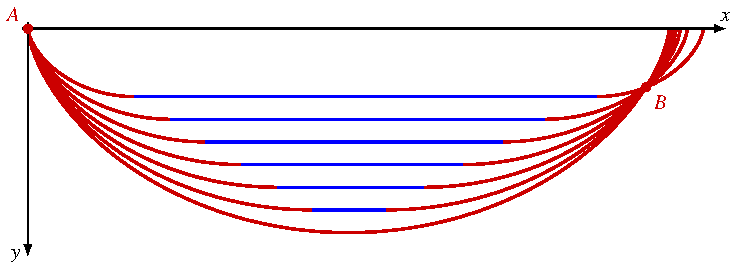
\includegraphics{chapters/020-variation/images/singulaer.pdf}
\caption{Verschiedene Lösungen des Brachistochronenproblems
unter Verwendung der singulären Lösungen
der Differentialgleichung der Brachistochronen.
Die roten Kurventeile sind Lösungen der ursprünglichen
Brachistochronengleichung
\eqref{buch:variation:eulerlagrange:eqn:brachistochrone0},
die blauen Teile sind durch die Multiplikation mit $y'$ in
\eqref{buch:variation:eulerlagrange:eqn:multiplikation}
hinzugekommen, sind aber nicht Lösungen der ursprünglichen
Gleichungen.
Nur die untereste Kurve ist daher eine Brachistochrone.
\label{buch:variation:eulerlagrange:fig:brachloes}}
\end{figure}
